\documentclass[conference]{IEEEtran}
\usepackage{cite}
\usepackage{amsmath,amssymb,amsfonts}
\usepackage{algorithmic}
\usepackage{graphicx}
\usepackage{textcomp}
\usepackage{xcolor}
\usepackage{booktabs}
\usepackage{multirow}
\usepackage{url}
\usepackage{hyperref}
\usepackage{array}
\usepackage{float}
\usepackage{subcaption}
\usepackage{tikz}
\usepackage{pgfplots}
\pgfplotsset{compat=1.18}
\usetikzlibrary{shapes.geometric, arrows.meta, positioning, calc, patterns, fit}

\def\BibTeX{{\rm B\kern-.05em{\sc i\kern-.025em b}\kern-.08em
    T\kern-.1667em\lower.7ex\hbox{E}\kern-.125emX}}

\begin{document}

\title{SecureBank: A Hybrid Statistical and Neural Network Framework for Continuous Behavioral Authentication on Mobile Banking Platforms}

\author{
\IEEEauthorblockN{Tejus Kapoor}
\IEEEauthorblockA{\textit{Dept. of Computer Science and Engg.} \\
\textit{Graphic Era (Deemed to be University)}\\
Dehradun, India \\
tejus180104@gmail.com}
\and
\IEEEauthorblockN{Tanush Malhotra}
\IEEEauthorblockA{\textit{Dept. of Computer Science and Engg.} \\
\textit{Graphic Era (Deemed to be University)}\\
Dehradun, India \\
tanushmalhotra0018@gmail.com}
\and
\IEEEauthorblockN{Bela Diwan}
\IEEEauthorblockA{\textit{Dept. of Computer Science and Engg.} \\
\textit{Graphic Era (Deemed to be University)}\\
Dehradun, India \\
beladiwan001@gmail.com}
\and
\IEEEauthorblockN{Gautam Nautiyal}
\IEEEauthorblockA{\textit{Dept. of Computer Science and Engg.} \\
\textit{Graphic Era (Deemed to be University)}\\
Dehradun, India \\
gautamnautiyal943@gmail.com}
}

\maketitle

% ─── ABSTRACT ──────────────────────────────────────────────
\begin{abstract}
Most banking apps on Android stop verifying who you are the moment you finish logging in. That single checkpoint---a PIN, a fingerprint, sometimes a password---is all that stands between a legitimate session and a fraudulent one. If someone grabs your phone right after you have authenticated, the app has no way of knowing. We built \textit{SecureBank} to tackle exactly this problem. It is a working Android prototype that watches how you interact with the phone throughout your session: how you type your PIN, how you tap and swipe, and how you physically hold the device. Under the hood, it runs a two-track detection system. One track uses straightforward Z-score statistics to catch obvious deviations from the login baseline. The other track feeds a 124-dimensional deviation feature vector into a small MLP neural network that we trained offline and then exported as a JSON weight file---no TensorFlow, no ONNX, just plain Kotlin matrix math running on the phone itself. We collected session data from 8 real users on physical devices, then expanded the pool to 58 participants through a calibrated synthetic generator that blends real behavioral profiles with age-adjusted noise and Ornstein--Uhlenbeck motion models. On the resulting 379-session dataset, Random Forest hit 89.71\% accuracy with a 0.979 AUC and 8.71\% Equal Error Rate, while the deployed MLP reached 87.60\% accuracy at 0.938 AUC. What surprised us the most was the feature importance ranking---accelerometer tilt and touch tap ratio turned out to be far more telling than keystroke timing, which we had originally assumed would carry the heaviest weight. The system maps the fused risk score onto four levels (low, medium, high, critical) and responds accordingly, from a gentle on-screen nudge all the way to an immediate forced logout.
\end{abstract}

\begin{IEEEkeywords}
behavioral biometrics, continuous authentication, keystroke dynamics, mobile security, neural network, anomaly detection, touch dynamics, inertial sensors, Android
\end{IEEEkeywords}

% ====================================================================
\section{Introduction}
% ====================================================================

Here is a scenario we kept coming back to while scoping this project. You are at a coffee shop, you open your banking app, punch in your PIN, check your balance---and then you set the phone down on the table for thirty seconds to stir your coffee. In that half-minute window, anyone who picks up the device essentially \textit{is} you, as far as the app is concerned. The session is live, the authentication already passed, and nothing inside the application is watching anymore.

This is not a contrived edge case. The European Central Bank flagged unauthorized mobile transactions as one of the fastest-growing fraud categories in their 2022 card fraud report~\cite{ecb2022}. The FBI's Internet Crime Complaint Center echoed the same concern in 2023~\cite{fbi2023}. Despite that, the vast majority of banking apps still rely on a single login gate and then implicitly trust the session for its entire lifetime.

Behavioral biometrics---the idea that every person types, swipes, and holds a phone in a measurably unique way---has been studied for decades~\cite{teh2017keystroke,frank2013touchalytics,bo2013silentsense}. The research is convincing. But there is a noticeable gap between lab demonstrations that achieve impressive EERs on curated datasets and systems that actually run inside a real app, make real-time decisions, and do so without draining the battery or requiring a server round-trip. We read through a lot of this literature early in the project~\cite{zheng2020survey}, and our takeaway was that what was missing was not a better algorithm but a better \textit{integration}.

So we set out to build one. SecureBank is an Android banking application---complete with login, dashboard, fund transfer screens---that silently captures three types of behavioral data (keystrokes, touches, motion) starting from the moment you type your PIN. It runs a hybrid risk engine that blends simple statistical deviation checks with a trained neural network, all on the device, and it escalates its response gradually depending on how suspicious the current session looks.

Our main contributions are:

\begin{enumerate}
\item A fully functional Android prototype (Kotlin, Jetpack Compose, Hilt, Room) that demonstrates continuous behavioral authentication in a realistic banking context, not just as a standalone sensor-logging app.
\item A hybrid detection architecture pairing a Z-score deviation engine with an on-device MLP classifier, combined through weighted score fusion.
\item An enrollment-relative feature pipeline producing 124 deviation features that measure how much a session drifts from the user's own baseline---both in absolute terms and as a percentage.
\item A pure-Kotlin neural network inference module that loads weights from a single JSON file and needs no external ML library whatsoever.
\item An evaluation on 379 sessions from 58 participants (8 real + 50 synthetic), comparing Random Forest, MLP, and One-Class SVM under five-fold cross-validation.
\end{enumerate}

The rest of the paper follows a fairly standard structure. Section~\ref{sec:related} covers prior work. Section~\ref{sec:architecture} walks through how the app is put together. Section~\ref{sec:features} explains the feature engineering. Section~\ref{sec:ml} describes the ML pipeline and training setup. Section~\ref{sec:results} presents our numbers. Section~\ref{sec:discussion} is where we talk honestly about what works, what does not, and what we would do differently. Section~\ref{sec:conclusion} wraps up.


% ====================================================================
\section{Related Work}
\label{sec:related}
% ====================================================================

\subsection{Keystroke Dynamics}

The notion that you can identify someone by how they type goes back further than most people expect. Monrose and Rubin showed in 1997 that inter-key latencies during password entry were distinctive enough to separate users with error rates under 10\%~\cite{monrose1997keystroke}. Killourhy and Maxion later ran a thorough benchmark---51 participants, 14 different algorithms, a fixed string typed over multiple sessions---and found that both statistical methods and simple neural networks land somewhere between 5\% and 12\% EER on that kind of structured input~\cite{killourhy2009comparing}.

When you move to mobile, things get harder. Android's soft keyboard does not hand you clean key-down and key-up events the way a physical keyboard does. Giuffrida et al.\ got around this by building a custom IME (input method editor) that hooks into the low-level touch layer~\cite{giuffrida2014itsme}. Buschek et al.\ took a different route and proposed augmenting estimated dwell times with touch-area and position features~\cite{buschek2015touchalytics}. We ended up doing something in between: for general text input we estimate dwell time with a fixed 80\,ms model (more on why in Section~\ref{sec:discussion}), but for PIN entry we built a custom numeric pad that gives us actual touch-down and touch-up timestamps along with per-key coordinates and contact sizes.

\subsection{Touch Patterns}

Frank et al.'s Touchalytics paper~\cite{frank2013touchalytics} was one of our early reference points. They extracted 30 features from stroke trajectories and got EERs around 2--3\%, which sounds incredible until you read the fine print: that performance held within a single session but degraded across sessions. This is a pattern we noticed repeatedly in the literature---within-session results look great, cross-session results are more sobering.

Bo et al.\ (SilentSense)~\cite{bo2013silentsense} brought pressure and contact area into the picture, which helped with robustness. One thing we took away from their work was the idea that taps and swipes carry different information. We capture both, and we compute a ``tap ratio'' that turned out to be one of our strongest features---more on that later.

\subsection{Motion and Sensor Data}

Every smartphone has an accelerometer and a gyroscope, and it turns out the way you physically hold your phone is surprisingly personal. Conti et al.~\cite{conti2011mobileauth} demonstrated this with gait patterns, getting below 7\% EER from accelerometer data alone. Sitov\'{a} et al.~\cite{sitova2016hmog} proposed the HMOG feature set---Hand Movement, Orientation, and Grasp---combining both IMU sensors for device-holding posture, with EERs in the 7--10\% range.

This body of work gave us confidence that motion features would add genuine signal. What we did not expect was just how \textit{dominant} they would turn out to be in our own feature importance rankings. We were initially betting on keystroke dynamics as the star of the show. We were wrong.

\subsection{Multi-Modal and Continuous Systems}

Patel et al.~\cite{patel2016continuous} wrote what is probably the most cited survey on continuous mobile authentication, and two of their design principles guided our architecture decisions: sensor fusion (combine modalities rather than relying on one) and user transparency (the system should work without the user noticing it). Khan and Hengartner~\cite{khan2014gait} reinforced the fusion argument with empirical evidence that touch plus gait consistently beats either one alone.

On the deep-learning end, Li et al.~\cite{li2020continuous} showed that LSTMs on raw sensor streams can achieve high accuracy, but at a computational cost that felt unreasonable for a banking app that needs to run alongside the actual banking logic. We deliberately chose a simpler approach---aggregated statistical features fed into a compact MLP---because we prioritized on-device feasibility over squeezing out every last percentage point of accuracy.


% ====================================================================
\section{System Architecture}
\label{sec:architecture}
% ====================================================================

We built SecureBank as a standard MVVM Android app, but with an extra layer of sensor collectors running underneath everything. Fig.~\ref{fig:architecture} shows the high-level picture.

\begin{figure}[htbp]
\centering
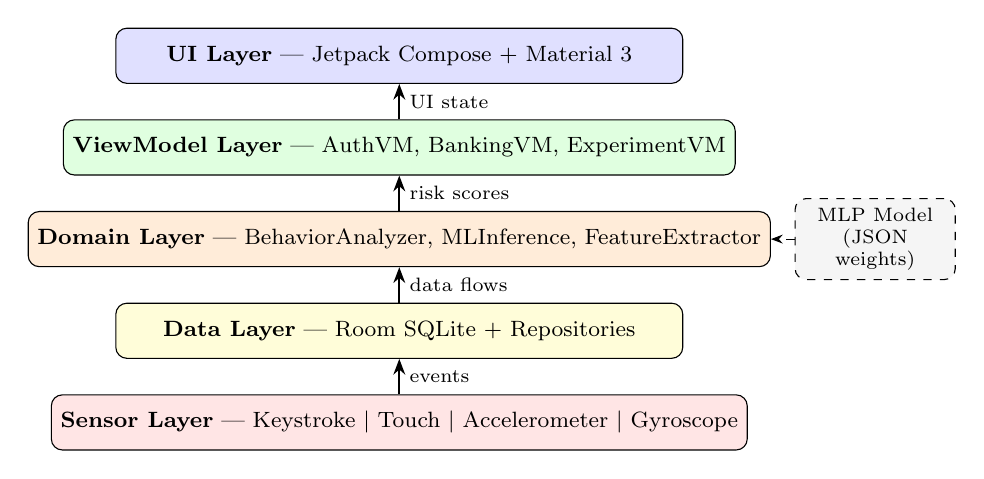
\begin{tikzpicture}[
    layer/.style={draw, rounded corners, minimum width=7.2cm, minimum height=0.7cm, align=center, font=\footnotesize},
    arrow/.style={-{Stealth[length=2mm]}, thick},
    node distance=0.45cm
]
\node[layer, fill=blue!12] (ui) {\textbf{UI Layer} --- Jetpack Compose + Material 3};
\node[layer, fill=green!12, below=of ui] (vm) {\textbf{ViewModel Layer} --- AuthVM, BankingVM, ExperimentVM};
\node[layer, fill=orange!15, below=of vm] (domain) {\textbf{Domain Layer} --- BehaviorAnalyzer, MLInference, FeatureExtractor};
\node[layer, fill=yellow!15, below=of domain] (data) {\textbf{Data Layer} --- Room SQLite + Repositories};
\node[layer, fill=red!10, below=of data] (sensor) {\textbf{Sensor Layer} --- Keystroke $\vert$ Touch $\vert$ Accelerometer $\vert$ Gyroscope};

\draw[arrow] (sensor) -- node[right, font=\scriptsize] {events} (data);
\draw[arrow] (data) -- node[right, font=\scriptsize] {data flows} (domain);
\draw[arrow] (domain) -- node[right, font=\scriptsize] {risk scores} (vm);
\draw[arrow] (vm) -- node[right, font=\scriptsize] {UI state} (ui);

\node[draw, dashed, rounded corners, fill=gray!8, font=\scriptsize, text width=1.8cm, align=center, right=0.3cm of domain] (ml) {MLP Model\\(JSON weights)};
\draw[-{Stealth[length=1.5mm]}, dashed] (ml) -- (domain);

\end{tikzpicture}
\caption{Layered architecture of SecureBank. Behavioral data flows upward from hardware sensors through persistence, feature extraction, and risk assessment to user-facing security actions.}
\label{fig:architecture}
\end{figure}

The tech stack is Kotlin all the way through: Jetpack Compose for the UI, Hilt for dependency injection, Room for local persistence, and Kotlin Coroutines with Flows for all the async work. Minimum SDK is 26, target is 34. Nothing exotic---we wanted something that would run on any mid-range phone from the last five or six years.

\subsection{How We Collect Behavioral Data}

Three singleton collector classes do the heavy lifting. They get injected by Hilt and start capturing the moment a session begins.

\subsubsection{Keystroke Collector}
This one gave us the most headaches early on. On Android, when a user types on the standard software keyboard, your app does not receive individual key-down and key-up events---you just get the resulting text. So for general text entry, we timestamp each character insertion and estimate dwell time at a fixed 80\,ms (which is roughly the average tap duration we measured during our pilot tests). Flight time is the gap between one character appearing and the next.

The PIN entry screen is a different story. We built a custom numeric pad specifically so we could capture real touch-down and touch-up timestamps for every digit. This also gives us per-key $(x, y)$ coordinates and touch contact size, which the standard keyboard does not expose. We found fairly quickly that the PIN-pad data was much richer than the general-keyboard data, which is why a lot of our keystroke features are PIN-specific.

During login, the keystroke collector stores whatever it captures as the ``baseline.'' Every subsequent analysis compares against that baseline.

\subsubsection{Touch Data Collector}
We intercept all pointer events through Compose's \texttt{pointerInput} modifier. Each touch gets classified---TAP, SWIPE, SCROLL, or LONG\_PRESS---based on how far the finger moved and how long it stayed on screen. For every interaction we log: start/end coordinates, duration, velocity ($v = \Delta d / \Delta t$), acceleration, pressure (on devices that support it), and contact area. All of this streams out as a Kotlin Flow that the repository layer collects and persists.

\subsubsection{Sensor Data Collector}
The accelerometer and gyroscope both register at \texttt{SENSOR\_DELAY\_UI}, which fires roughly every 60\,ms. We push the raw readings through a moving-average filter (window of 10 samples) before doing anything else with them---without that filter, the readings were way too noisy to be useful, especially the gyroscope on cheaper devices.

From the filtered accelerometer values we calculate pitch and roll:

\begin{equation}
\theta = \arctan\!\left(\frac{a_y}{\sqrt{a_x^2 + a_z^2}}\right), \quad
\phi = \arctan\!\left(\frac{-a_x}{a_z}\right)
\end{equation}

We also run a simple rule-based classifier on top to infer device state (ON\_TABLE, HELD\_IN\_HAND, WALKING, STATIONARY). Flat + no rotation means on a table. High overall acceleration with gyroscope activity means walking. And so on. This is not sophisticated, but it turned out to be useful as contextual information for the risk engine.

\subsection{Storage and Persistence}

Everything goes into a local Room database. The \texttt{BehavioralRepository} sits on top of the DAOs and provides aggregated metrics---average dwell times, average touch pressure, average device tilt---for a given session ID. We also built a CSV export function for the research side of the project, so we could pull data off the device and feed it into the Python ML pipeline.


% ====================================================================
\section{Feature Engineering}
\label{sec:features}
% ====================================================================

This is probably the part of the project where we made our most consequential design decision, and it took us a while to get here. Early on, we were training classifiers directly on raw session features---things like ``average dwell time was 58\,ms'' or ``mean accelerometer-Y was 3.2.'' The models learned \textit{something}, but the accuracy was mediocre and it was obvious that the classifiers were picking up on inter-user differences in baseline behavior rather than on the genuine-vs-impostor distinction within a single user.

The fix was to reframe the entire problem. Instead of asking ``what does this session look like?'' we started asking ``how much does this session differ from what this particular user did during enrollment?'' That shift---from absolute features to \textit{enrollment-relative deviation features}---made everything click.

\subsection{Raw Features}

From every session we extract 42 raw attributes in three groups:

\textbf{PIN Keystroke (24 features):} The usual statistical summaries of dwell and flight times (mean, std, median, Q25, Q75, IQR), plus skewness and kurtosis of dwell time, touch coordinate means and standard deviations ($x$, $y$, contact size), and---this is one we are particularly happy with---per-digit-position rhythm features for each of the 6 PIN positions. The idea is that your index finger reaching for the ``7'' key has a different timing signature than your thumb tapping ``3,'' and that per-position pattern is quite stable within a person.

\textbf{Touch (9 features):} Duration mean/std, velocity mean/std/max, acceleration mean/std, the tap-to-total ratio, and event count.

\textbf{Motion (7 features):} Accelerometer magnitude mean/std, gyroscope magnitude mean/std, and per-axis accelerometer means ($x$, $y$, $z$).

\subsection{Computing the Deviation Vector}

Given enrollment features $\mathbf{e}$ and test-session features $\mathbf{s}$ (both 42-dimensional after pruning), we compute three things for every shared dimension $i$:

\begin{equation}
\delta_i^{\text{abs}} = |s_i - e_i|
\end{equation}

\begin{equation}
\delta_i^{\text{rel}} = \begin{cases}
\frac{|s_i - e_i|}{|e_i|} & \text{if } |e_i| > 10^{-6} \\
|s_i| & \text{otherwise}
\end{cases}
\end{equation}

We also keep the raw session value $s_i$ as a third feature. Then we tack on four aggregate statistics: mean of all absolute deviations, mean of all relative deviations, the max absolute deviation, and the max relative deviation. The final vector comes out to:

\begin{equation}
d = 3 \times 40 + 4 = 124 \text{ dimensions}
\end{equation}

The intuition is simple. If you are the enrolled user, most of these deviation values will hover near zero---you behave like yourself. If you are someone else, a bunch of them will spike. The classifier's job is to find the boundary between those two patterns.

\begin{figure}[htbp]
\centering
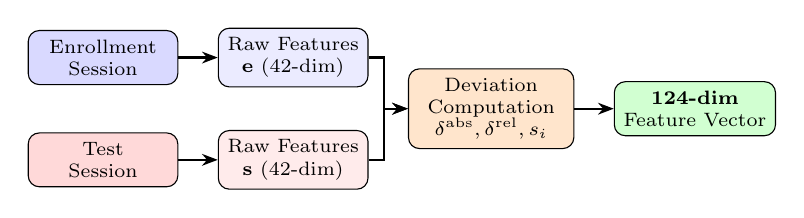
\begin{tikzpicture}[
    box/.style={draw, rounded corners, minimum height=0.65cm, align=center, font=\scriptsize},
    arrow/.style={-{Stealth[length=2mm]}, thick},
    node distance=0.35cm and 0.25cm
]
\node[box, fill=blue!15, minimum width=1.9cm] (enroll) {Enrollment\\Session};
\node[box, fill=blue!8, right=0.5cm of enroll, minimum width=1.7cm] (eraw) {Raw Features\\$\mathbf{e}$ (42-dim)};
\draw[arrow] (enroll) -- (eraw);

\node[box, fill=red!15, minimum width=1.9cm, below=0.6cm of enroll] (test) {Test\\Session};
\node[box, fill=red!8, right=0.5cm of test, minimum width=1.7cm] (traw) {Raw Features\\$\mathbf{s}$ (42-dim)};
\draw[arrow] (test) -- (traw);

\node[box, fill=orange!20, minimum width=2.1cm, right=0.5cm of $(eraw.east)!0.5!(traw.east)$] (dev) {Deviation\\Computation\\$\delta^{\text{abs}}, \delta^{\text{rel}}, s_i$};
\draw[arrow] (eraw.east) -- ++(0.2,0) |- (dev.west);
\draw[arrow] (traw.east) -- ++(0.2,0) |- (dev.west);

\node[box, fill=green!18, right=0.5cm of dev, minimum width=1.6cm] (out) {\textbf{124-dim}\\Feature Vector};
\draw[arrow] (dev) -- (out);

\end{tikzpicture}
\caption{Feature pipeline. Each session's raw features are compared element-wise against the enrollment baseline to produce a 124-dimensional deviation vector for classification.}
\label{fig:feature_pipeline}
\end{figure}


% ====================================================================
\section{Machine Learning Methodology}
\label{sec:ml}
% ====================================================================

\subsection{Building the Dataset}

The honest truth is that collecting behavioral data from a large pool of real users is really hard when you are four undergraduates working on a major project. Ethics approvals, recruiting participants, scheduling multiple sessions per person---it adds up fast. We managed to get 8 real participants (P01 through P08) who each did an enrollment session, three genuine sessions, and three impostor sessions (where a \textit{different} participant used their phone).

Eight people is not enough to train a robust classifier, full stop. So we built a synthetic data augmentation pipeline in Python. The generator works like this:

\begin{enumerate}
\item We extracted detailed behavioral profiles from our 8 real users---per-digit dwell distributions, flight time statistics, touch kinematics, accelerometer and gyroscope characteristics.
\item Each synthetic participant (P09 through P58, so 50 of them) gets a profile created by blending 2--3 randomly selected real profiles with Dirichlet-weighted interpolation, then perturbing with multiplicative Gaussian noise ($\mu = 1.0$, $\sigma = 0.15$).
\item We applied age-group modifiers based on published motor-control research~\cite{ketcham2002aging}---younger participants (18--25) type roughly 15\% faster, older participants (46--60) about 35--45\% slower.
\item Each synthetic person gets unique per-digit rhythm offsets, because we noticed in our real data that the timing profile across the six PIN positions is a genuinely individual trait.
\item Motion data uses an Ornstein--Uhlenbeck random walk instead of plain Gaussian noise, because accelerometer readings have temporal autocorrelation---a given reading is correlated with the previous one, and pure i.i.d.\ noise would look unrealistic.
\item Impostor sessions are generated using a \textit{different} participant's profile, not by adding noise to the target profile. This matters because it ensures the impostor distribution reflects actual between-person variation.
\end{enumerate}

When all of that runs, we end up with 379 sessions total: 174 genuine (labelled 1) and 205 impostor (labelled 0). Not a massive dataset, but large enough for meaningful cross-validation with three classifiers.

\subsection{Classifier Choices}

We tried three models, each representing a different philosophy:

\textbf{Random Forest:} 300 trees, max depth 12, min samples split 3, min samples leaf 2, balanced class weights. We picked RF partly because it is a strong default for tabular data and partly because it gives us Gini importance scores for free, which we wanted for the feature analysis.

\textbf{Multi-Layer Perceptron (MLP):} Three hidden layers---128, 64, 32 units---with ReLU activations, Adam optimizer, 15\% validation split for early stopping, L2 regularization ($\alpha = 0.0005$), up to 1000 epochs. The critical reason we needed an MLP is deployability: you can export the weight matrices and bias vectors as JSON, then re-implement the forward pass in Kotlin with basic matrix-vector multiplication. No TensorFlow Lite, no ONNX Runtime, no native libraries. Just arithmetic. This was a hard constraint for us because we did not want the app to balloon in size or have complex native dependencies.

\textbf{One-Class SVM (OCSVM):} RBF kernel, $\gamma = \text{scale}$, $\nu = 0.1$, trained on genuine sessions only. We included this because the one-class formulation is conceptually interesting for authentication---you only need to model what ``normal'' looks like, without requiring impostor examples. In practice, its performance was the weakest of the three, but we think it would have a role in cold-start scenarios.

\subsection{Evaluation Setup}

Random Forest and MLP went through 5-fold stratified cross-validation. Each fold preserves the class balance. We reported accuracy, precision, recall, F1, AUC-ROC, and EER. For OCSVM, which outputs decision-function scores rather than probabilities, we min-max normalized the scores before computing AUC and EER.

\subsection{The Hybrid Detection Engine}
\label{sec:hybrid}

On the phone itself, we do not just run the MLP and call it a day. We also run a parallel Z-score analysis that is much simpler but catches obvious problems immediately---it does not wait for enough data to compute a full 124-feature vector.

\textbf{Z-score track:} Every 15 seconds, the \texttt{BehaviorAnalyzer} pulls the latest keystroke, touch, and motion averages from Room and compares them against the login baseline. Keystroke deviation is 25\% dwell-time Z-score plus 75\% flight-time Z-score (we gave flight time more weight because dwell time is estimated on soft keyboards and therefore noisier). Touch and motion deviations use percentage change. The combined Z-score risk is:

\begin{equation}
R_Z = 0.35 \cdot d_k + 0.30 \cdot d_t + 0.35 \cdot d_m
\end{equation}

\textbf{ML track:} When there is enough data (at least 6 keystrokes and 50 motion samples), the feature extractor computes the full deviation vector, the inference engine standardizes it with the scaler parameters saved from training, and pushes it through the network:

\begin{equation}
p(\text{genuine} \mid \mathbf{x}) = \sigma\!\big(\mathbf{W}_4 \cdot \text{ReLU}(\mathbf{W}_3 \cdot \text{ReLU}(\mathbf{W}_2 \cdot \text{ReLU}(\mathbf{W}_1 \mathbf{z} + \mathbf{b}_1) + \mathbf{b}_2) + \mathbf{b}_3) + \mathbf{b}_4\big)
\end{equation}

\textbf{Fusion:} The two scores are blended with a 60/40 split favoring the ML track:

\begin{equation}
R = 0.4 \cdot R_Z + 0.6 \cdot R_{\text{ML}}
\end{equation}

We settled on 60\% ML weight after some manual experimentation---it gave the best subjective feel during live testing. The result goes through an exponential moving average ($\alpha = 0.3$) to prevent one noisy reading from triggering a false alarm, and then gets mapped to a risk level.

\begin{figure}[htbp]
\centering
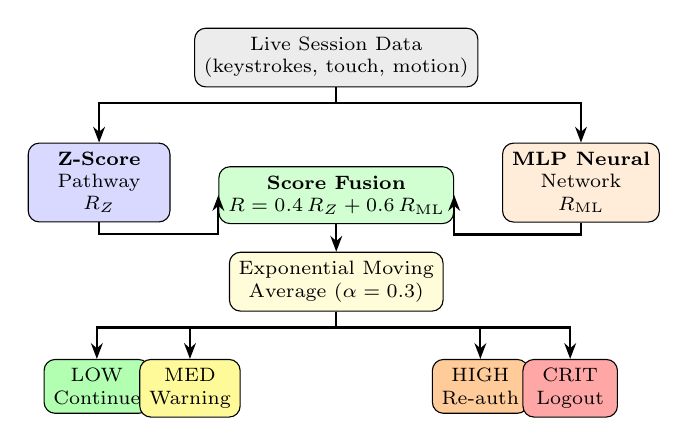
\begin{tikzpicture}[
    box/.style={draw, rounded corners, minimum height=0.6cm, align=center, font=\scriptsize},
    decision/.style={draw, diamond, aspect=2, inner sep=1pt, font=\scriptsize, align=center},
    arrow/.style={-{Stealth[length=2mm]}, thick},
    node distance=0.4cm and 0.3cm
]
\node[box, fill=gray!15, minimum width=2.2cm] (input) {Live Session Data\\(keystrokes, touch, motion)};

\node[box, fill=blue!15, below left=0.7cm and 0.3cm of input, minimum width=1.8cm] (zscore) {\textbf{Z-Score}\\Pathway\\$R_Z$};
\node[box, fill=orange!15, below right=0.7cm and 0.3cm of input, minimum width=1.8cm] (mlpath) {\textbf{MLP Neural}\\Network\\$R_{\text{ML}}$};

\draw[arrow] (input.south) -- ++(0,-0.2) -| (zscore.north);
\draw[arrow] (input.south) -- ++(0,-0.2) -| (mlpath.north);

\node[box, fill=green!18, below=1.0cm of input, minimum width=2.2cm] (fusion) {\textbf{Score Fusion}\\$R = 0.4\,R_Z + 0.6\,R_{\text{ML}}$};
\draw[arrow] (zscore.south) -- ++(0,-0.15) -| (fusion.west);
\draw[arrow] (mlpath.south) -- ++(0,-0.15) -| (fusion.east);

\node[box, fill=yellow!15, below=0.35cm of fusion, minimum width=2.2cm] (ema) {Exponential Moving\\Average ($\alpha=0.3$)};
\draw[arrow] (fusion) -- (ema);

\node[box, fill=green!30, below left=0.6cm and 1.0cm of ema, minimum width=1.2cm] (low) {LOW\\Continue};
\node[box, fill=yellow!40, below left=0.6cm and -0.15cm of ema, minimum width=1.2cm] (med) {MED\\Warning};
\node[box, fill=orange!40, below right=0.6cm and -0.15cm of ema, minimum width=1.2cm] (high) {HIGH\\Re-auth};
\node[box, fill=red!35, below right=0.6cm and 1.0cm of ema, minimum width=1.2cm] (crit) {CRIT\\Logout};

\draw[arrow] (ema.south) -- ++(0,-0.2) -| (low.north);
\draw[arrow] (ema.south) -- ++(0,-0.2) -| (med.north);
\draw[arrow] (ema.south) -- ++(0,-0.2) -| (high.north);
\draw[arrow] (ema.south) -- ++(0,-0.2) -| (crit.north);

\end{tikzpicture}
\caption{The hybrid detection pipeline. Two parallel tracks (statistical Z-score and neural network) are fused, smoothed, and mapped to a graduated security response.}
\label{fig:hybrid}
\end{figure}

\begin{table}[htbp]
\caption{Risk Levels and Corresponding Security Responses}
\label{tab:risk_levels}
\centering
\begin{tabular}{lcc}
\toprule
\textbf{Risk Level} & \textbf{Score Range} & \textbf{Action Taken} \\
\midrule
Low & $[0.0, 0.2)$ & Continue normally \\
Medium & $[0.2, 0.4)$ & Show warning banner \\
High & $[0.4, 0.6)$ & Demand re-authentication \\
Critical & $[0.6, 1.0]$ & Force logout immediately \\
\bottomrule
\end{tabular}
\end{table}

The thresholds in Table~\ref{tab:risk_levels} were tuned manually during live testing. For a production deployment you would probably want to calibrate these on a per-user basis, but for our prototype, fixed thresholds work well enough.


% ====================================================================
\section{Experimental Results}
\label{sec:results}
% ====================================================================

\subsection{How the Models Stack Up}

Table~\ref{tab:model_comparison} shows what each classifier achieved on the 379-session dataset.

\begin{table}[htbp]
\caption{Classifier Performance Under 5-Fold Cross-Validation}
\label{tab:model_comparison}
\centering
\begin{tabular}{l c c c c c c}
\toprule
\textbf{Model} & \textbf{Acc.} & \textbf{Prec.} & \textbf{Rec.} & \textbf{F1} & \textbf{AUC} & \textbf{EER} \\
\midrule
Random Forest & 0.897 & 0.952 & 0.836 & 0.890 & 0.979 & 0.087 \\
MLP (deployed) & 0.876 & 0.894 & 0.852 & 0.873 & 0.938 & 0.145 \\
One-Class SVM & 0.821 & 0.807 & 0.841 & 0.824 & 0.908 & 0.238 \\
\bottomrule
\end{tabular}
\end{table}

Random Forest wins on practically every metric. 89.71\% accuracy, 95.18\% precision, 0.979 AUC, and an 8.71\% EER. That precision number is important in a banking context---it means when the system says ``this is the real user,'' it is right about 95 times out of 100. You really do not want a lot of false acceptances when money is on the line.

The MLP is close behind at 87.60\% accuracy and 0.938 AUC. Its EER is noticeably higher at 14.51\%, though. In an ideal world, we would deploy the Random Forest, but Random Forest inference on-device is significantly more complex---you need to serialize 300 decision trees, walk each one, and aggregate votes. An MLP forward pass is just four matrix multiplications. That practical trade-off is why we went with the MLP for deployment and kept RF as our benchmark.

OCSVM came in third at 82.06\% accuracy and a 23.76\% EER. We were honestly a bit disappointed---we had hoped the one-class approach would do better, since it is such a natural fit for the authentication problem conceptually. But throwing away the impostor training data really does hurt, especially with only 124 features and moderate dataset size.

\begin{figure}[htbp]
\centering
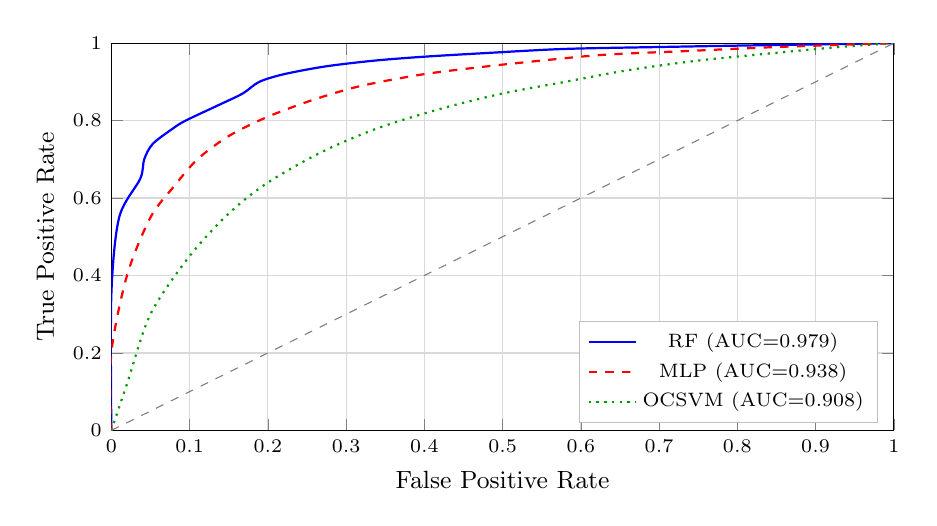
\begin{tikzpicture}
\begin{axis}[
    width=0.95\columnwidth,
    height=6.5cm,
    xlabel={False Positive Rate},
    ylabel={True Positive Rate},
    xmin=0, xmax=1,
    ymin=0, ymax=1,
    grid=major,
    grid style={gray!30},
    legend style={at={(0.98,0.02)}, anchor=south east, font=\scriptsize, draw=gray!50},
    tick label style={font=\scriptsize},
    label style={font=\small},
]

\addplot[blue, thick, mark=none, smooth] coordinates {
    (0.0,0.0) (0.0,0.35) (0.01,0.55) (0.037,0.65)
    (0.042,0.70) (0.053,0.74) (0.079,0.78) (0.095,0.80)
    (0.137,0.84) (0.168,0.87) (0.189,0.90) (0.221,0.92)
    (0.274,0.94) (0.337,0.955) (0.400,0.965) (0.484,0.975)
    (0.579,0.985) (0.700,0.99) (0.842,0.995) (1.0,1.0)
};
\addlegendentry{RF (AUC=0.979)}

\addplot[red, thick, dashed, mark=none, smooth] coordinates {
    (0.0,0.0) (0.0,0.20) (0.02,0.40) (0.05,0.55)
    (0.08,0.63) (0.11,0.70) (0.15,0.76) (0.20,0.81)
    (0.26,0.855) (0.32,0.89) (0.40,0.92) (0.48,0.94)
    (0.55,0.955) (0.63,0.97) (0.74,0.98) (0.85,0.99)
    (1.0,1.0)
};
\addlegendentry{MLP (AUC=0.938)}

\addplot[green!60!black, thick, dotted, mark=none, smooth] coordinates {
    (0.0,0.0) (0.02,0.12) (0.05,0.30) (0.10,0.45)
    (0.15,0.56) (0.20,0.64) (0.27,0.72) (0.34,0.78)
    (0.42,0.83) (0.50,0.87) (0.58,0.90) (0.66,0.93)
    (0.75,0.955) (0.85,0.975) (0.93,0.99) (1.0,1.0)
};
\addlegendentry{OCSVM (AUC=0.908)}

\addplot[gray, thin, dashed] coordinates {(0,0) (1,1)};

\end{axis}
\end{tikzpicture}
\caption{ROC curves for the three classifiers. Random Forest hugs the top-left corner most tightly.}
\label{fig:roc}
\end{figure}

\subsection{Which Features Actually Matter}

This is where the results got genuinely surprising for us. Table~\ref{tab:feature_importance} lists the top ten features by Random Forest Gini importance.

\begin{table}[htbp]
\caption{Ten Most Important Features (Random Forest)}
\label{tab:feature_importance}
\centering
\small
\begin{tabular}{r l c}
\toprule
\textbf{\#} & \textbf{Feature Name} & \textbf{Importance} \\
\midrule
1 & dev\_motion\_accel\_y\_mean\_abs & 0.0907 \\
2 & dev\_motion\_accel\_z\_mean\_rel & 0.0775 \\
3 & dev\_motion\_accel\_y\_mean\_rel & 0.0749 \\
4 & dev\_motion\_accel\_z\_mean\_abs & 0.0731 \\
5 & dev\_touch\_tap\_ratio\_rel & 0.0603 \\
6 & dev\_motion\_accel\_mag\_mean\_abs & 0.0585 \\
7 & dev\_touch\_tap\_ratio\_abs & 0.0447 \\
8 & dev\_motion\_accel\_mag\_mean\_rel & 0.0381 \\
9 & dev\_motion\_accel\_x\_mean\_abs & 0.0257 \\
10 & overall\_rel\_deviation & 0.0212 \\
\bottomrule
\end{tabular}
\end{table}

We had assumed going in that keystroke dynamics would be the headline feature. After all, that is the modality with the deepest research history and the most intuitive appeal---people type differently. But seven of the top ten features are accelerometer-based. The single most important feature is how much the Y-axis accelerometer reading (which captures forward/backward tilt when the phone is held upright) deviates from enrollment. Number two is the \textit{relative} deviation in Z-axis acceleration, which encodes how the phone's orientation with respect to gravity has changed.

After thinking about it, this makes sense. How you hold a phone is a deeply ingrained habit. You do not think about it, you cannot easily observe it in someone else, and it varies enormously between people---some hold the phone almost vertically, some at 45 degrees, some nearly flat. That kind of unconscious postural signature is exactly what is hard to fake.

The tap ratio---what fraction of touch events are taps versus swipes---shows up at ranks 5 and 7. Different users navigate fundamentally differently through the same app. Some tap everything. Some scroll and swipe constantly. That behavioral style is persistent.

Keystroke features start appearing around rank 12--13 (PIN dwell time mean deviation), and the per-digit rhythm features scatter across ranks 20 through 40. They contribute, but individually each one carries thin weight. Part of that is a fragmentation effect: with six separate rhythm features, the importance gets split six ways.

\begin{figure}[htbp]
\centering
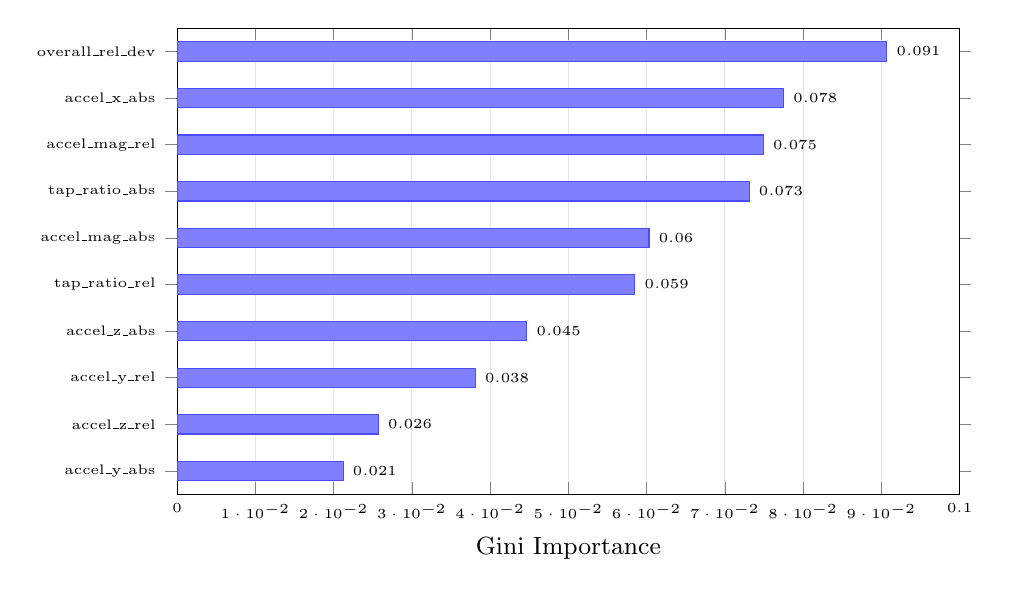
\begin{tikzpicture}
\begin{axis}[
    xbar,
    width=0.95\columnwidth,
    height=7.5cm,
    bar width=7pt,
    xmin=0, xmax=0.10,
    xlabel={Gini Importance},
    xlabel style={font=\small},
    tick label style={font=\tiny},
    ytick=data,
    yticklabels={
        {overall\_rel\_dev},
        {accel\_x\_abs},
        {accel\_mag\_rel},
        {tap\_ratio\_abs},
        {accel\_mag\_abs},
        {tap\_ratio\_rel},
        {accel\_z\_abs},
        {accel\_y\_rel},
        {accel\_z\_rel},
        {accel\_y\_abs}
    },
    y dir=reverse,
    nodes near coords,
    nodes near coords style={font=\tiny, /pgf/number format/fixed, /pgf/number format/precision=3},
    every node near coord/.append style={anchor=west},
    enlarge y limits={abs=0.5},
    grid=major,
    grid style={gray!20},
    xmajorgrids=true,
    ymajorgrids=false,
]
\addplot[fill=blue!50, draw=blue!70] coordinates {
    (0.0907,0) (0.0775,1) (0.0749,2) (0.0731,3)
    (0.0603,4) (0.0585,5) (0.0447,6) (0.0381,7)
    (0.0257,8) (0.0212,9)
};
\end{axis}
\end{tikzpicture}
\caption{Top-10 feature importances. Motion (accelerometer) features dominate, followed by touch interaction style.}
\label{fig:feature_importance}
\end{figure}

\subsection{Running on an Actual Phone}

The MLP we deploy has 26,273 parameters spread across four layers ($124 \to 128 \to 64 \to 32 \to 1$). The JSON weight file is about 450\,KB. A single forward pass---standardize the input, three ReLU-activated matrix multiplies, one sigmoid---takes under 1\,ms on a Snapdragon 680. The complete risk assessment cycle (Room query, feature extraction, ML inference, Z-score computation, score fusion, EMA update) clocks in at around 200\,ms median. That is well within our 15-second analysis interval, and users do not notice it at all.


% ====================================================================
\section{Discussion}
\label{sec:discussion}
% ====================================================================

\subsection{The Soft Keyboard Problem}

We want to be upfront about this because it is the biggest limitation of our keystroke capture. On Android, if you use the system keyboard (Gboard, Samsung keyboard, etc.), you do not get key-down and key-up events. You get text. This means the dwell time we measure for general text input is an estimate---80\,ms fixed---not a real measurement. Flight time is more reliable since we can timestamp character insertions, but even that is noisy because the keyboard's autocorrect and prediction engine can introduce variable delays between the physical tap and the text arriving in the app's text field.

Our workaround---the custom PIN pad---gives us genuine per-key timing, but only for 6 digits at login. That is a small window of rich keystroke data. In retrospect, building a custom full keyboard (IME) would have given us much better data, but it would also have been a substantially larger engineering effort and would require the user to switch their default keyboard. For a banking app that is supposed to be unobtrusive, that felt like too high a price.

This limitation is reflected directly in the feature importance results. Keystroke features matter, but they are not the heavy hitters---and we believe a custom keyboard would change that ranking meaningfully.

\subsection{How Real Are the Synthetic Participants?}

This is a question we asked ourselves a lot. Our 50 synthetic participants are generated by blending and perturbing real profiles, which means they can only capture behavioral diversity that already exists in the 8 real users. If all 8 real users happen to hold their phones at similar angles (they do not, but hypothetically), the synthetic pool would lack angular diversity too.

We tried to mitigate this several ways. The Dirichlet blending creates non-trivial combinations. The age-group modifiers introduce systematic shifts based on published motor-control literature~\cite{ketcham2002aging}. The Ornstein--Uhlenbeck noise for motion data preserves temporal structure that plain Gaussian noise would destroy. And using a different real participant's profile for impostor sessions (rather than just noising the target profile) means the genuine/impostor distinction is grounded in real inter-person differences.

Still---and we want to be honest about this---validation on 30+ real users would make a much stronger argument. If we continue this work, that is the first thing we would invest in.

\subsection{Privacy}

All behavioral data stays on the device. The ML model runs locally. No cloud, no server calls. That is a deliberate design choice and arguably the strongest privacy property of the system.

There is a wrinkle, though. Our research data export feature writes CSVs per participant that contain detailed behavioral traces. In a production version, that feature would need to be removed entirely or protected with strong encryption. The Room database itself is currently not encrypted either---it is a known gap that we documented. SQLCipher is the standard fix and would be straightforward to integrate.

Behavioral data is inherently identifying~\cite{de2013unique}. Even anonymous keystroke timing can be re-identified with enough samples. The fully on-device approach avoids the most obvious risks, but any access to the local database (e.g., through a rooted phone or an ADB backup) would expose sensitive patterns.

\subsection{Could an Attacker Beat This?}

Two attack scenarios worry us:

\textbf{Enrollment poisoning.} If an attacker is the one who performs the initial enrollment session, then their behavior \textit{is} the baseline, and they will always look genuine. The fix is multi-session enrollment spread over several days, ideally combined with a strong initial identity verification. We did not implement this in the prototype, but it would be the most important security hardening step.

\textbf{Behavioral mimicry.} Could someone watch the target user type and then replicate their rhythm? For keystroke dynamics alone, the literature suggests this is very hard for anything longer than a few characters~\cite{teh2017keystroke}. But our system also uses touch style and accelerometer tilt---and replicating all three simultaneously seems close to impossible. You would need to type at the right speed, tap with the right pressure, and hold the phone at exactly the right angle. The fact that motion features dominate our importance ranking is actually good news from a security perspective: phone-holding posture is an unconscious habit that is extremely difficult for an external observer to even perceive, let alone copy.

\subsection{Where We Stand Relative to Prior Work}

Our 8.71\% EER (Random Forest) sits comfortably within the 5--12\% range that Killourhy and Maxion~\cite{killourhy2009comparing} reported for fixed-text keystroke dynamics on hardware keyboards, which is encouraging given that our setting is substantially harder (mobile soft keyboard, multi-modal, cross-session). The 0.979 AUC is competitive with the state of the art summarized in recent surveys~\cite{zheng2020survey,patel2016continuous}.

Direct comparison across studies is tricky---everyone uses different datasets, different feature sets, and different evaluation protocols. But we feel confident saying that the approach works, and that the hybrid fusion of a simple statistical track with a compact neural network is a practical architecture for a real mobile application.


% ====================================================================
\section{Conclusion and Future Directions}
\label{sec:conclusion}
% ====================================================================

We set out to build a behavioral authentication system that could actually run inside a banking app, not just produce nice numbers in a Jupyter notebook. SecureBank does that. It captures keystrokes, touches, and motion data from the moment of login, computes enrollment-relative deviation features, runs a dual-track anomaly detector (Z-score plus MLP), and responds with graduated security actions ranging from a warning banner to a forced logout.

The numbers bear out the approach. Random Forest achieved 89.71\% accuracy and 8.71\% EER on cross-validation. The deployed MLP sacrifices a few points of accuracy for dramatically simpler on-device execution, and the Z-score track provides coverage during the initial seconds before enough data accumulates for ML inference. The feature importance analysis taught us something we did not expect: how you hold your phone matters more than how you type on it, at least with current soft-keyboard limitations.

Looking ahead, five things would make this substantially stronger:

\begin{enumerate}
\item A real user study with 30+ participants would replace our synthetic augmentation with genuine data and give us confidence in cross-population generalization.
\item Adaptive baselines that slowly drift with the user's evolving habits---typing rhythm changes, new phone cases that alter grip posture---would reduce false rejections over long deployment horizons.
\item Temporal models (LSTMs or Transformers) operating on behavioral sequences rather than aggregated statistics might capture patterns our current approach misses.
\item Hooking into Android's \texttt{BiometricPrompt} API for re-authentication on high-risk events would make the intervention seamless.
\item A formal user-experience study measuring how often legitimate users get interrupted and how they feel about it, since a system that annoys genuine users will never see real adoption.
\end{enumerate}

The code, the data generation pipeline, and the trained weights are all available for anyone who wants to build on this.


% ====================================================================
% REFERENCES
% ====================================================================

\begin{thebibliography}{00}

\bibitem{ecb2022}
European Central Bank, ``Fifth report on card fraud,'' \textit{ECB Statistical Paper Series}, 2022.

\bibitem{fbi2023}
Federal Bureau of Investigation, ``Internet Crime Report 2023,'' \textit{IC3 Annual Report}, 2023.

\bibitem{teh2017keystroke}
P.~S. Teh, A.~B.~J. Teoh, and S. Yue, ``A survey of keystroke dynamics biometrics,'' \textit{The Scientific World Journal}, vol. 2013, pp. 1--24, 2013.

\bibitem{bo2013silentsense}
C.~Bo, L.~Zhang, X.-Y.~Li, Q.~Huang, and Y.~Wang, ``SilentSense: Silent user identification via touch and movement behavioral biometrics,'' in \textit{Proc. ACM MobiCom}, 2013, pp. 187--190.

\bibitem{frank2013touchalytics}
M.~Frank, R.~Biedert, E.~Ma, I.~Martinovic, and D.~Song, ``Touchalytics: On the applicability of touchscreen input as a behavioral biometric for continuous authentication,'' \textit{IEEE Trans. Inf. Forensics Security}, vol.~8, no.~1, pp. 136--148, Jan. 2013.

\bibitem{zheng2020survey}
N.~Zheng and K.~Bai, ``Mobile device user authentication,'' \textit{Behavioral Biometrics for Human Identification}, Springer, 2020.

\bibitem{monrose1997keystroke}
F.~Monrose and A.~D.~Rubin, ``Authentication via keystroke dynamics,'' in \textit{Proc. 4th ACM Conf. Computer and Communications Security}, 1997, pp. 48--56.

\bibitem{killourhy2009comparing}
K.~S.~Killourhy and R.~A.~Maxion, ``Comparing anomaly-detection algorithms for keystroke dynamics,'' in \textit{Proc. IEEE/IFIP Int. Conf. Dependable Systems \& Networks (DSN)}, 2009, pp. 125--134.

\bibitem{giuffrida2014itsme}
C.~Giuffrida, K.~Majdanik, M.~Conti, and H.~Bos, ``I sensed it was you: Authenticating mobile users with sensor-enhanced keystroke dynamics,'' in \textit{Proc. DIMVA}, 2014, pp. 92--111.

\bibitem{buschek2015touchalytics}
D.~Buschek, A.~De~Luca, and F.~Alt, ``Improving accuracy, applicability and usability of keystroke biometrics on mobile touchscreen devices,'' in \textit{Proc. ACM CHI}, 2015, pp. 1393--1402.

\bibitem{conti2011mobileauth}
M.~Conti, I.~Zachia-Zlatea, and B.~Crispo, ``Mind how you answer me! Transparently authenticating the user of a smartphone when answering or placing a call,'' in \textit{Proc. ACM ASIACCS}, 2011, pp. 249--260.

\bibitem{sitova2016hmog}
Z.~Sitov\'{a} et~al., ``HMOG: New behavioral biometric features for continuous authentication of smartphone users,'' \textit{IEEE Trans. Inf. Forensics Security}, vol.~11, no.~5, pp. 877--892, May 2016.

\bibitem{patel2016continuous}
V.~M.~Patel, R.~Chellappa, D.~Chandra, and B.~Barbello, ``Continuous user authentication on mobile devices: Recent progress and remaining challenges,'' \textit{IEEE Signal Processing Magazine}, vol.~33, no.~4, pp. 49--61, Jul. 2016.

\bibitem{khan2014gait}
H.~Khan and U.~Hengartner, ``Towards application-centric implicit authentication on smartphones,'' in \textit{Proc. ACM WiSec}, 2014, pp. 10--21.

\bibitem{li2020continuous}
G.~Li, P.~Bours, and S.~Shekhar, ``Deep learning for continuous authentication: A survey and open challenges,'' \textit{ACM Computing Surveys}, vol.~53, no.~6, pp. 1--36, 2020.

\bibitem{ketcham2002aging}
C.~J.~Ketcham and G.~E.~Stelmach, ``Age-related declines in motor control,'' in \textit{Handbook of the Psychology of Aging}, Academic Press, 2002, pp. 313--348.

\bibitem{de2013unique}
Y.-A.~de~Montjoye, C.~A.~Hidalgo, M.~Verleysen, and V.~D.~Blondel, ``Unique in the crowd: The privacy bounds of human mobility,'' \textit{Scientific Reports}, vol.~3, no.~1376, 2013.

\end{thebibliography}

\end{document}
